%!TEX root = ../deco_star.tex

%-------------------------------------------------------------------------
\section{Designs and Models}


\subsection{Design Goals}
\label{sec:design_goals}

In the pervious section we have discussed how creativity could be enabled, in the following section we highlight to which type of pattern designs such an enabling of creative creation could lead.

\question[inline]{We do need to introduce and elaborate what we mean with "creative" here?!}

% For this investigation of control mechanisms for pattern generation, we +
The survey of creative pattern generation triggers challenging questions in regard to the specific design goals. The investigated design goals go beyond the basic repetition of elements to create patterns. Creative pattern generation requires both, the application of formative design principles as well as creative freedom for artists.

For a better understanding of the required design principles, we define ornamentation as aspired design goal, derive design principles from that goal and investigate techniques towards that goal.

The Oxford English Dictionary~\cite{oed_2017} defines ornaments as nonessential accessories intended to adorn. There is no functionality to an ornament other than to beautify a manufactured article without changing its shape or character~\cite{ward_1896_tpo}. The term ornament can be found in a large variety of contexts, such as in architecture, music or poetry, but this work only refers to two-dimensional visual ornaments. While ornaments may carry symbolic meanings in the arranged elements \cite{wornum_1896_aof}, this work does not include semantics but focuses on visual qualities.

Different cultures and times resulted in various ornamental styles, with great differences in the details as \Cref{fig:historic_examples} shows. Nevertheless common underlying design principles for ornamentation can be identified.

\begin{figure}
    % \centering
       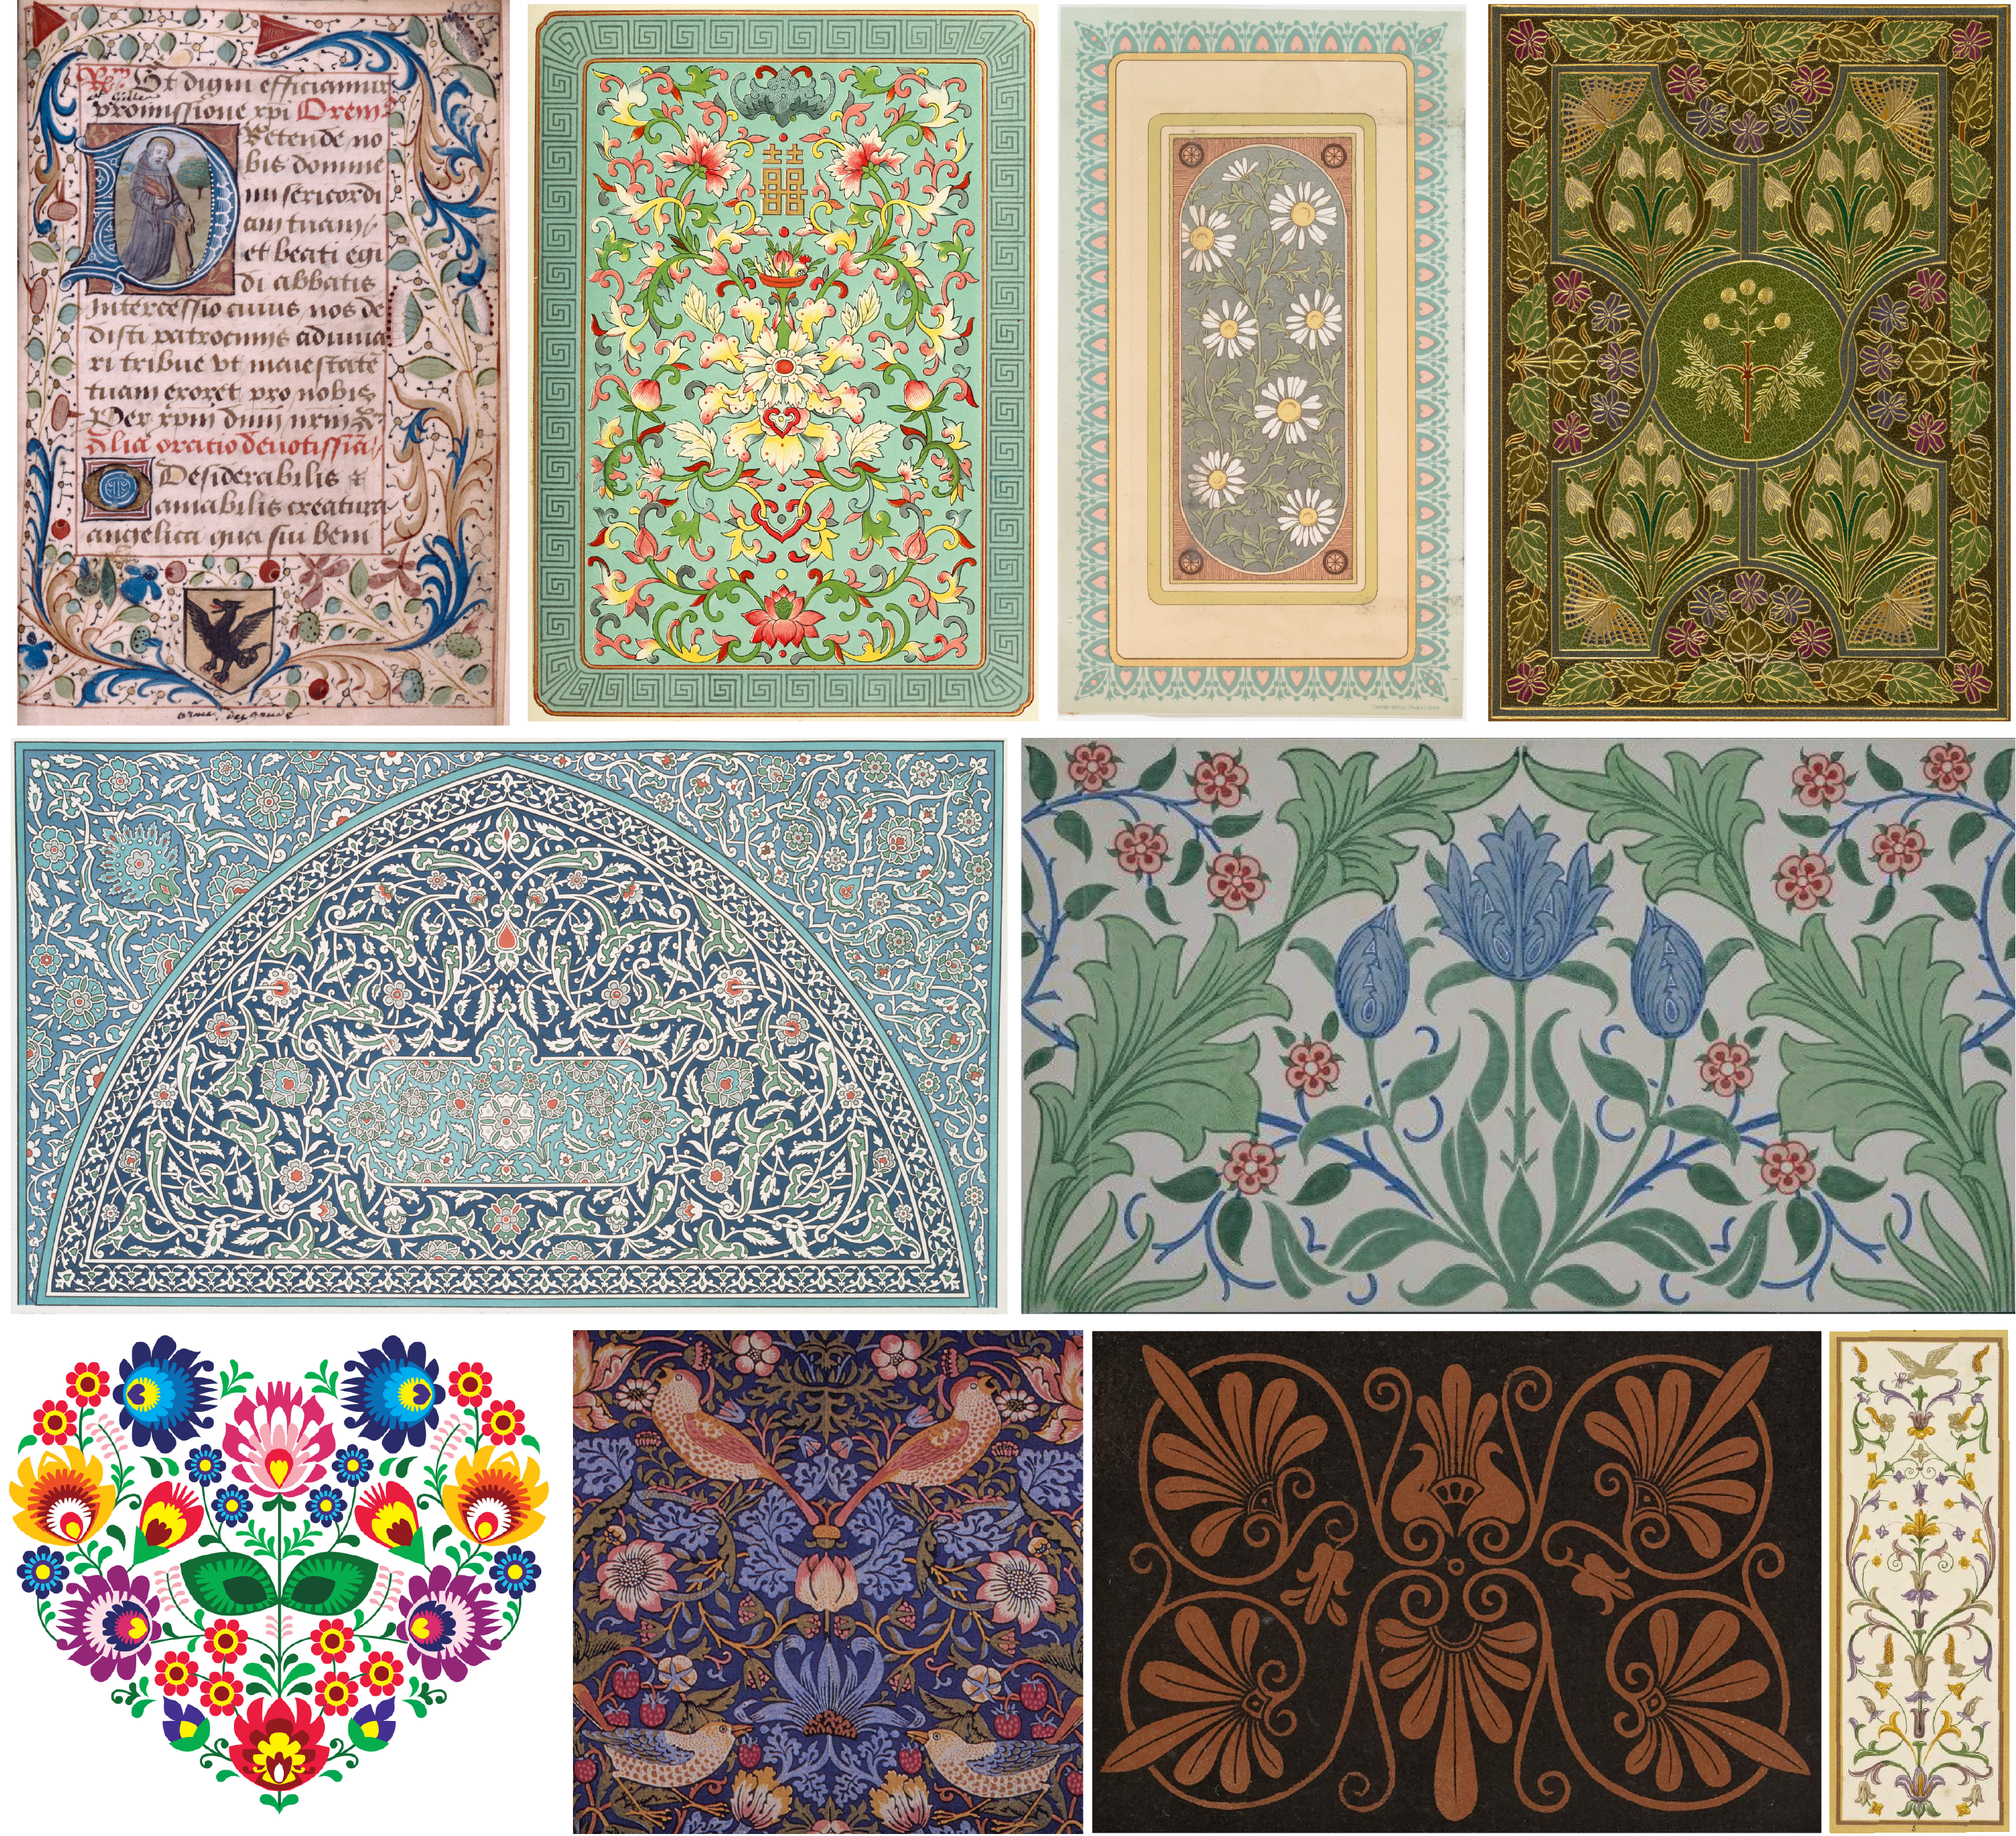
\includegraphics[width=1.0\columnwidth]{figures/historic_examples/historic_examples.png}
        \caption[Historic ornamentation examples]{\label{fig:historic_examples} Historic ornamentation examples. Places of origin from left to right, top to bottom:  France, China, USA, UK, Egypt, UK$^{*}$, Poland, UK$^{*}$, Greece, Italy. $^{*}$Images are cutouts of tiled pattern but are often found as presented here. Image sources: please refer to~\Cref{chap:img_refs_taxo}~\nameref{chap:img_refs}.}
\end{figure}

Ornamentation can be understood as an accurately defined type of decor that follows a structural logic~\cite{ward_1896_tpo, moughtin_1999_udo, arbruzzo_2006_dec}. 
% But the transition between formal ornamentation and informal decoration is smooth, with various common aspects~\cite{moughtin_1999_udo}. 
In addition to its aesthetic appeal, an ornament is perceptually distinguished by a sense of order and by its alignment to the space it fills (as summarized by \citeauthor*{wong_1998_cgf}~\cite{wong_1998_cgf} and originally stated by \citeauthor*{ward_1896_tpo}~\cite{ward_1896_tpo, dresser_1875_pdd, arbruzzo_2006_dec}). 
 \citeauthor*{arbruzzo_2006_dec}~\cite{arbruzzo_2006_dec} elaborate on ornamentation as follows:

\begin{quote}
\textit{[An] ornament is inextricable linked to scale and proportion, to form and order. In this context, the modus operandi of ornamentation is always to reinforce an existing order: to conform to its partner in the ornament-object relationship, for ornament always has a partner in that which is ornamented.}
\end{quote}

An underlying perception of order in an ornament is established by even repetition and a balanced distribution of elements, with an intentionally designed and artificial quality~\cite{ward_1896_tpo}. Balance can be achieved with a careful composition of elements, and such balance is built on symmetrical arrangements in most ornaments. Compositions are not limited to the repetition of the same element, but different visual qualities can create various relationships. Visual characteristics attract the eye differently and the \textit{visual weight} of a feature can be used as a measure for the degree of attraction. For example, large, dark and highly saturated colored elements have a greater visual weight than small, light and desaturated ones. These visual weights can be used to create visual correlations (for example, based on Gestalt psychology - a topic too wide for a discussion here) and can counterbalance each other. A larger and lighter colored element might have the same visual weight as a smaller, darker colored one. Hence, varied elements with different visual properties can be combined and still make a balanced whole.


\begin{figure}
    % \centering
       \includegraphics[width=1\columnwidth]{figures/ornament/ornament_principles.pdf}
        \caption[Ornamentation principles]{\label{fig:ornamentation_principles} Exemplary dissection of visual characteristics fulfilling ornamental principles. Single features often support several principles, as, for example, the frames and borders create a hierarchical composition, an adaption to the space the ornament fills and visual contrasts. Image source: \cite{morris_1910_tol}.}
\end{figure}

Hierarchical compositions further increase a sense of order but are also used for creating contrasts (e.g., foreground vs. background) and accentuating structures (e.g., framing). These structures are often used to elaborate and accentuate the form of the space they fill, hence building the ornament-object relationship described by \citeauthor*{arbruzzo_2006_dec}~\cite{arbruzzo_2006_dec}. The following differentiation of an ornamental decoration gives an intuitive understanding of this aspect~\cite{arbruzzo_2006_dec}: Wallpaper can be trimmed for different rooms, but the design is not reproportioned or altered. An ornament, however, is fitted to and references the logic of the space it is designed for. Without adjustment, it cannot be transferred to a different space.

Contrasts and accents are crucial for the visual appeal of an ornament~\cite{wong_1998_cgf,ward_1896_tpo, moughtin_1999_udo}. Single, visually dominant elements and structures might not follow the underlying order of the ornament at all, breaking an otherwise too homogeneous appearance - again distinguishing ornamentation from wallpaper.

\Cref{fig:ornamentation_principles} gives an example of how the described design principles are combine seamlessly into a coherent design.

It takes artistic expertise to balance the contrast between carefully chosen visual accents and to create a sense of order by applying compositional rules and by complementing the space. However, it is exactly this combination of qualities - rule-based composition and repetition on the one hand and the placement of visual accents and the breaking free from order on the other - that make ornamentation an interesting but highly challenging field of algorithmic research in the context of computer graphics.

Ornamentation exemplifies the common challenge of enabling control for tasks for which humans are indispensable in combination with the automation of tedious manufacturing and the computation of structuring rules. With that it is a representative design goal to aspire to for an general investigation of creative control mechanisms.



% \subsubsection{Summary}
% \label{subsec:ornamentation_summary}

% \label{sum:ornamentation}
% \textit{Ornamentation}
%     \begin{itemize}
%     \item Perception of order
%     \item Hierarchical compositions
%     \item Adaptation to the space
%     \item Contrasts and visual accents
%     \end{itemize}



\subsection{Models}
\label{sec:models}

In the context of computer graphics, generation techniques are differentiated into procedural and data-driven approaches. This understanding applies equally to the generation of geometry, animations and texture, for example. 
% Through the continuous development of both fields, approaches started to blend and the advantages of both approaches are brought together. 
Procedural techniques describe the visual output by evaluating an algorithm, while data-driven approaches rely on existing data, such as photographs.
 
The underlying regularity of an ornament is based on a repetitive and balanced distribution of elements, usually following hierarchical structures. These characteristics can be efficiently implemented by procedural approaches \cite{stava_2010_ipm} because they automatically fill a space based on generative rules. An artist should be freed from such tedious, non-inspiring and repetitive tasks. In order to execute order, computational generation techniques are not only an easement, but they also perform in a potentially more precise and less error-prone way than a human artist. Hence, procedural representations are an ideal basis for ornamentation. However, the creative demands of laying out space-specific designs and of placing highlights must also be considered. Procedural models must be augmented, and different approaches must be unified in order to enable the control and quality of manual creation as well as the efficiency and accuracy of computation. For this goal, this survey focuses on procedural models as a basis, but it also integrates and highlights promising or desirable characteristics of suitable data-driven techniques.

The following categorizes \textit{procedural} models as \textit{stochastic}, \textit{function-} and \textit{rule-based}, \textit{grammar-based}, \textit{simulation-based}, and \textit{artificial intelligence-based}. A \textit{data-driven} approach is discussed, and models specifically developed for \textit{ornamental} designs are summarized.


\subsection{Procedural}
\label{subsec:models_procedural}
 \citeauthor*{ebert_2003_tmp}~\cite{ebert_2003_tmp} describe procedural techniques as algorithms and mathematical functions that synthesize a model or an effect.

Solely equation-based representations are considered the ``purest'' form of procedural modeling~\cite{smelik_2014_aso}. This approach gained immediate importance in the early days of computer graphics. Simple equations are able to reproduce many natural phenomena – such as wood, stone, water, smoke and plants – with only some lines of code in the range of kilobytes, hence being memory efficient. The main appeals of such procedural representation include its compactness in combination with being continuous, scalable and unbound to a specific resolution. While procedural generation techniques have been a constant basis for generating content for games, its characteristics of memory efficiency and unlimited resolution are more important than ever with the rise of virtual reality.

The compactness and efficiency of a procedural model also enable parameterization, resulting in the model being responsive and flexible. Parameters usually represent certain visual characteristics and their amplification. Parameterization brings the crucial benefit that, for example, textures remain editable throughout the entire visual effect production pipeline.

However, the effectiveness of traditional parameterization in helping an artist fulfill design goals is debatable. \citeauthor*{ebert_2003_tmp}~\cite{ebert_2003_tmp} argue that parameterization brings the benefit of a few parameters controlling large amounts of details. At the same time, this is potentially problematic for the realization of specific designs because these often require full individual control of all visual elements. Additionally, parameters are often non-intuitive due to representing overly abstract characteristics of the underlying functions and having overlapping effects~\cite{bourque_2004_ptm,lagae_2010_pis,gilet_2010_ias,benes_2011_gpm,lasram_2012_ssf,lasram_2012_ptp}.

In addition to the disadvantage in the control of a procedural representation, the creation of the representation itself, the procedural model, requires considerable effort – even though it is only a one-time investment. For the appearance of a model, the focus usually lies on a more generic design, like a texture class. For procedural textures specifically, handling antialiasing efficiently can also be challenging. For a valuable and in-detail survey of function-based design principles of procedural models with focus on textures, the interested reader is referred to \citeauthor*{ebert_2003_tmp}~\cite{ebert_2003_tmp}. 

Procedural models are not limited to purely function-based designs. For example, the pioneering work of \citeauthor*{Prusinkiewicz_2012_TAB}~\cite{Prusinkiewicz_2012_TAB} applies the grammar-based L-system to algorithmically model plant growth, an approach extensively investigated by the computer graphics community and considered as procedural.

The following classification of core mechanisms for procedural generation is based on the taxonomy of \citeauthor*{hendrikx_2013_pcg}~\cite{hendrikx_2013_pcg} for procedural content generation in the context of games and the categorization of \citeauthor*{smelik_2014_aso}~\cite{smelik_2014_aso} for procedural modeling for virtual worlds.


\subsubsection{Stochastic Models}
\label{subsubsec:models_stochastic}

For stochastic models, noise functions generate maps of random values. They can either be used in their original form as procedural model or as a basis function. Visual features can be added by combining multiple layers of the noise in different resolutions.

Perlin noise~\cite{perlin_1985_ais} is one of the most well known noise functions and can be used to directly create many natural phenomena. Typical noise functions are lattice value noise, lattice gradient noise (e.g., Perlin noise), sparse convolution noise and spectral noise~\cite{ebert_2003_tmp,lagae_2010_sap}. These ``pure'' procedural programs also have the advantage of being well suited for optimization, such as parallelization, because they can be randomly evaluated in constant time~\cite{lagae_2010_sap}.

In the context of creative control for ornamentation, stochastic models build a basis for many designs but their design spectrum and controllability are limited.


\subsubsection{Function- and Rule-based Models}
\label{subsubsec:models_function}

Function-based models extend the class of stochastic models by layering and combining a variety of functions to form a visually complex pattern. Typical building blocks are periodic, spline, step, clamp and conditional functions~\cite{ebert_2003_tmp}. 

Rule-based models are part of individual, and often quite complex, generation systems that can be context-dependent and/or design-specific. Rule-based models are programs that relate to and partition the space to fill and follow propagation rules. The algorithmic core often handles proxy shapes, while for the result graphical elements, such as vector graphics, are mapped to the proxies.

Rule-based procedural models are the most suitable for ornamentation and novel control mechanisms because their iterative generation logic is the most open and flexible~\cite{wong_1998_cgf, mech_2012_tdf}. They can implement any designs and include any elements. Moreover, within a suitable pipeline, they can potentially take global constraints into consideration and build structural hierarchies.


\subsubsection{Grammar-based Models}
\label{subsubsec:models_grammar}

Grammar-based models are also considered ``purely'' procedural~\cite{smelik_2014_aso}. These models form grammatically-correct sentences from individual words, based on a system of rules. Originally introduced in theoretical linguistics by Noam Chomsky in the late 1950s, grammars are applied in computer graphics to generate objects such as plants from elements encoded as letters or words~\cite{hendrikx_2013_pcg}. Prominent techniques are L-systems and shape grammars. An emerging subgroup of grammar-based models includes \textit{probabilistic} inference into the derivation of correct sentences from a grammar.

In recent years, there have been a variety of successful grammar-based approaches for certain aspects of ornamentation~\cite{benes_2011_gpm,talton_2011_mpm,ritchie_2015_cpm}. However, grammars are difficult to set up and to design~\cite{stava_2010_ipm}. Because the execution process is inherently hierarchical, grammar systems have difficulty in supporting creative control from a global to local scale.

\subsubsection{Simulation Models}
\label{subsubsec:models_simulation}

Simulation models are based on techniques that approximate complex phenomena for which an analytical solution is unmanageable or unavailable. \citeauthor*{hendrikx_2013_pcg}~\cite{hendrikx_2013_pcg} further group simulation techniques into cellular automata, vector and tensor fields, and agent-based simulations. 

In the context of ornamentation, simulation models have been less relevant, with the exception of vector and tensor fields~\cite{ijiri_2008_aeb,yuanyuan_2011_gso,saputra_2017_ffo}. For simulation models usually interactive performance is a challenge, as well as the control on an element level. However, the potential to create a layout within a space and adapt to the characteristics of that space within a simulation system as well as the possible design variability call for further investigation.


\subsubsection{Artificial Intelligence Models}
\label{subsubsec:models_ai}

Artificial intelligence models represent approaches that go beyond the direct execution of specific rules. For example, they automatically optimize results based on fitness or error functions, or they apply planning steps. \citeauthor*{hendrikx_2013_pcg}~\cite{hendrikx_2013_pcg} group this class into genetic algorithms, neural networks and constraint satisfaction and planning. 

In recent years, machine learning has been introduced into procedural content generation with the same impact as in all other computer science fields~\cite{summerville_2017_pcg}. The potential of machine learning techniques in regard to creative control and ornamentation seems almost limitless and is further discussed as outlook of the chapter (\Cref{subsubsec:outlook_machinelearning}~\nameref{subsubsec:outlook_machinelearning}).


% \subsubsection{Summary}
% \label{subsubsec:models_summary}

% \begin{cframed}
% \textit{Procedural Models}
%     \begin{itemize}
%     \item Stochastic: maps of random values
%     \item Functions and Rules: partition and fill a space
%     \item Grammars: substitution system of rules and elements
%     \item Simulation: approximation of complex generation systems or phenomena
%     \item Artificial Intelligence: planning, adaptation and optimization 
%     \end{itemize}
% \end{cframed}



\subsection[Data-Driven]{Data-Driven Models}
\label{subsec:design_models_datadriven}

In contrast to procedural techniques, data-driven methods can be used in two ways in the context of ornamentation. First, they describe the processing of input pixel data, such as a photograph. Second, they refer to the output of a method, which is again pixel data. Data-driven models traditionally do not include underlying design models, as procedural representations do. Consequently, data-driven approaches are flexible in terms of possible designs and can achieve photorealism by processing real photographs.

At the same time, photographs bring the disadvantage of potentially including visual features, such as illumination effects, which are unwanted and difficult to remove. Moreover, further down a production pipeline, pixel data is usually not editable anymore. Working with data such as high-resolution images leads to high memory requirements, and without additional algorithms, data is fixed to its given resolution and scale.

% Does this section really fit here?
Addressing the issue of resolution example-based synthesis is a well established field of research and aims to create infinite amounts of pixel data based on a given exemplar. The pyramid-based texture synthesis of \citeauthor*{heeger_1995_pbt}~\cite{heeger_1995_pbt} is an early famous example.~\citeauthor*{wei_2009_seb}~\cite{wei_2009_seb} present a comprehensive summary of such example-based texture synthesis techniques, discussing statistical feature matching, neighborhood matching, patch-based and optimization methods. Overall, example-based methods for texture synthesis have achieved similar results in data size, random accessibility and editing and resolution options as procedural textures - but only within specialized contexts and not in an unified manner. Procedural textures offer these capabilities as inherent and combined characteristics.

Data-driven models are numerous and diverse because they can use and produce any input and output data without an underlying procedural model. Their classification is out of scope of this work. However, we do include in the following various techniques that offer further meaningful control mechanisms in the context of ornamentation. These techniques include the tiling and distribution of elements and drawing and brush mechanisms.

% For a review of models that output ornamental patterns, we focus on the output of the models and not on their underlying generation principles in order to come to a summarization.
